\documentclass[aspectratio=169]{beamer}
\usepackage{color,amsmath}
\usepackage{subfigure}
\usepackage{booktabs}
\usepackage{framed}
\usepackage{comment}

\def\vf{\vfill}

%%%%%%%%%%%%%%%%%%%%%%%%%%
\title[]{Big data\\(02-02)}
\author[]{Matthew J. Salganik\\Department of Sociology\\Princeton University}
\date[]{Soc 596: Computational Social Science\\Fall 2016
\vfill
\begin{flushright}
\vspace{0.6in}

\includegraphics[width=0.1\textwidth]{figures/cc.png}
\end{flushright}
}
\begin{document}
%%%%%%%%%%%%%%%%%%%%%%%%%%
\frame{\titlepage}
%%%%%%%%%%%%%%%%%%%%%%%%%%
\begin{frame}

\begin{itemize}
\item Observing behavior
\item Asking questions
\item Running experiments
\item Mass collaboration
\end{itemize}

\end{frame}
%%%%%%%%%%%%%%%%%%%%%%%%%%
\begin{frame}

{\Large
\begin{center}
What is big data?
\end{center}
}
\vf
Ambiguity makes a big tent

\end{frame}
%%%%%%%%%%%%%%%%%%%%%%%%%%
\begin{frame}

Big data:
\begin{itemize}
\item Volume
\item Velocity
\item Variety
\end{itemize}
\vf
Definition originates from business (Gartner)

\end{frame}
%%%%%%%%%%%%%%%%%%%%%%%%%%
\begin{frame}

Big data $\rightarrow$ repurposed data
\pause
\begin{itemize}
\item Business administrative data
\item Government administrative data
\end{itemize}

\end{frame}
%%%%%%%%%%%%%%%%%%%%%%%%%%
\begin{frame}

Big data $\rightarrow$ repurposed data
\pause
\begin{itemize}
\item good things
\item bad things
\end{itemize}

\end{frame}
%%%%%%%%%%%%%%%%%%%%%%%%%%\begin{frame}
\begin{frame}

Problems with the chapter:
\begin{itemize}
\item not all observed behavior is repurposed data, but most is
\item this is kind of residual category (not surveys, not experiments, not mass collaboration)
\end{itemize}

\end{frame}
%%%%%%%%%%%%%%%%%%%%%%%%%%
\begin{frame}

General advice:
\begin{itemize}
\item Imagine the ideal data.  How does your data compare?
\pause
\item Understand the data generating process (sometimes require reverse engineering goals of data creators)
\pause
\item Remember big data is not all of computational social science
\end{itemize}

\end{frame}
%%%%%%%%%%%%%%%%%%%%%%%%%%
\begin{frame}

\begin{center}
\begin{tabular}{ccc}
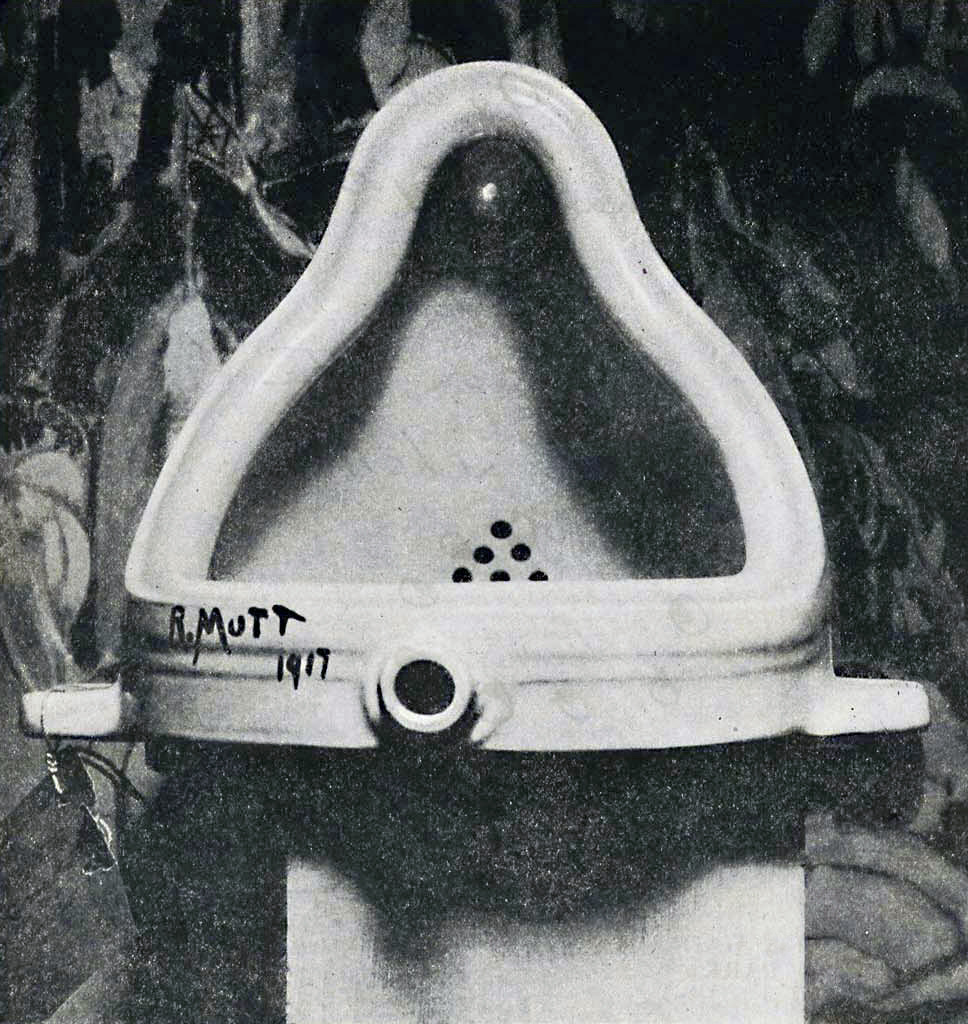
\includegraphics[width=0.30\textwidth]{figures/duchamp_fountain} & \phantom{12345} & 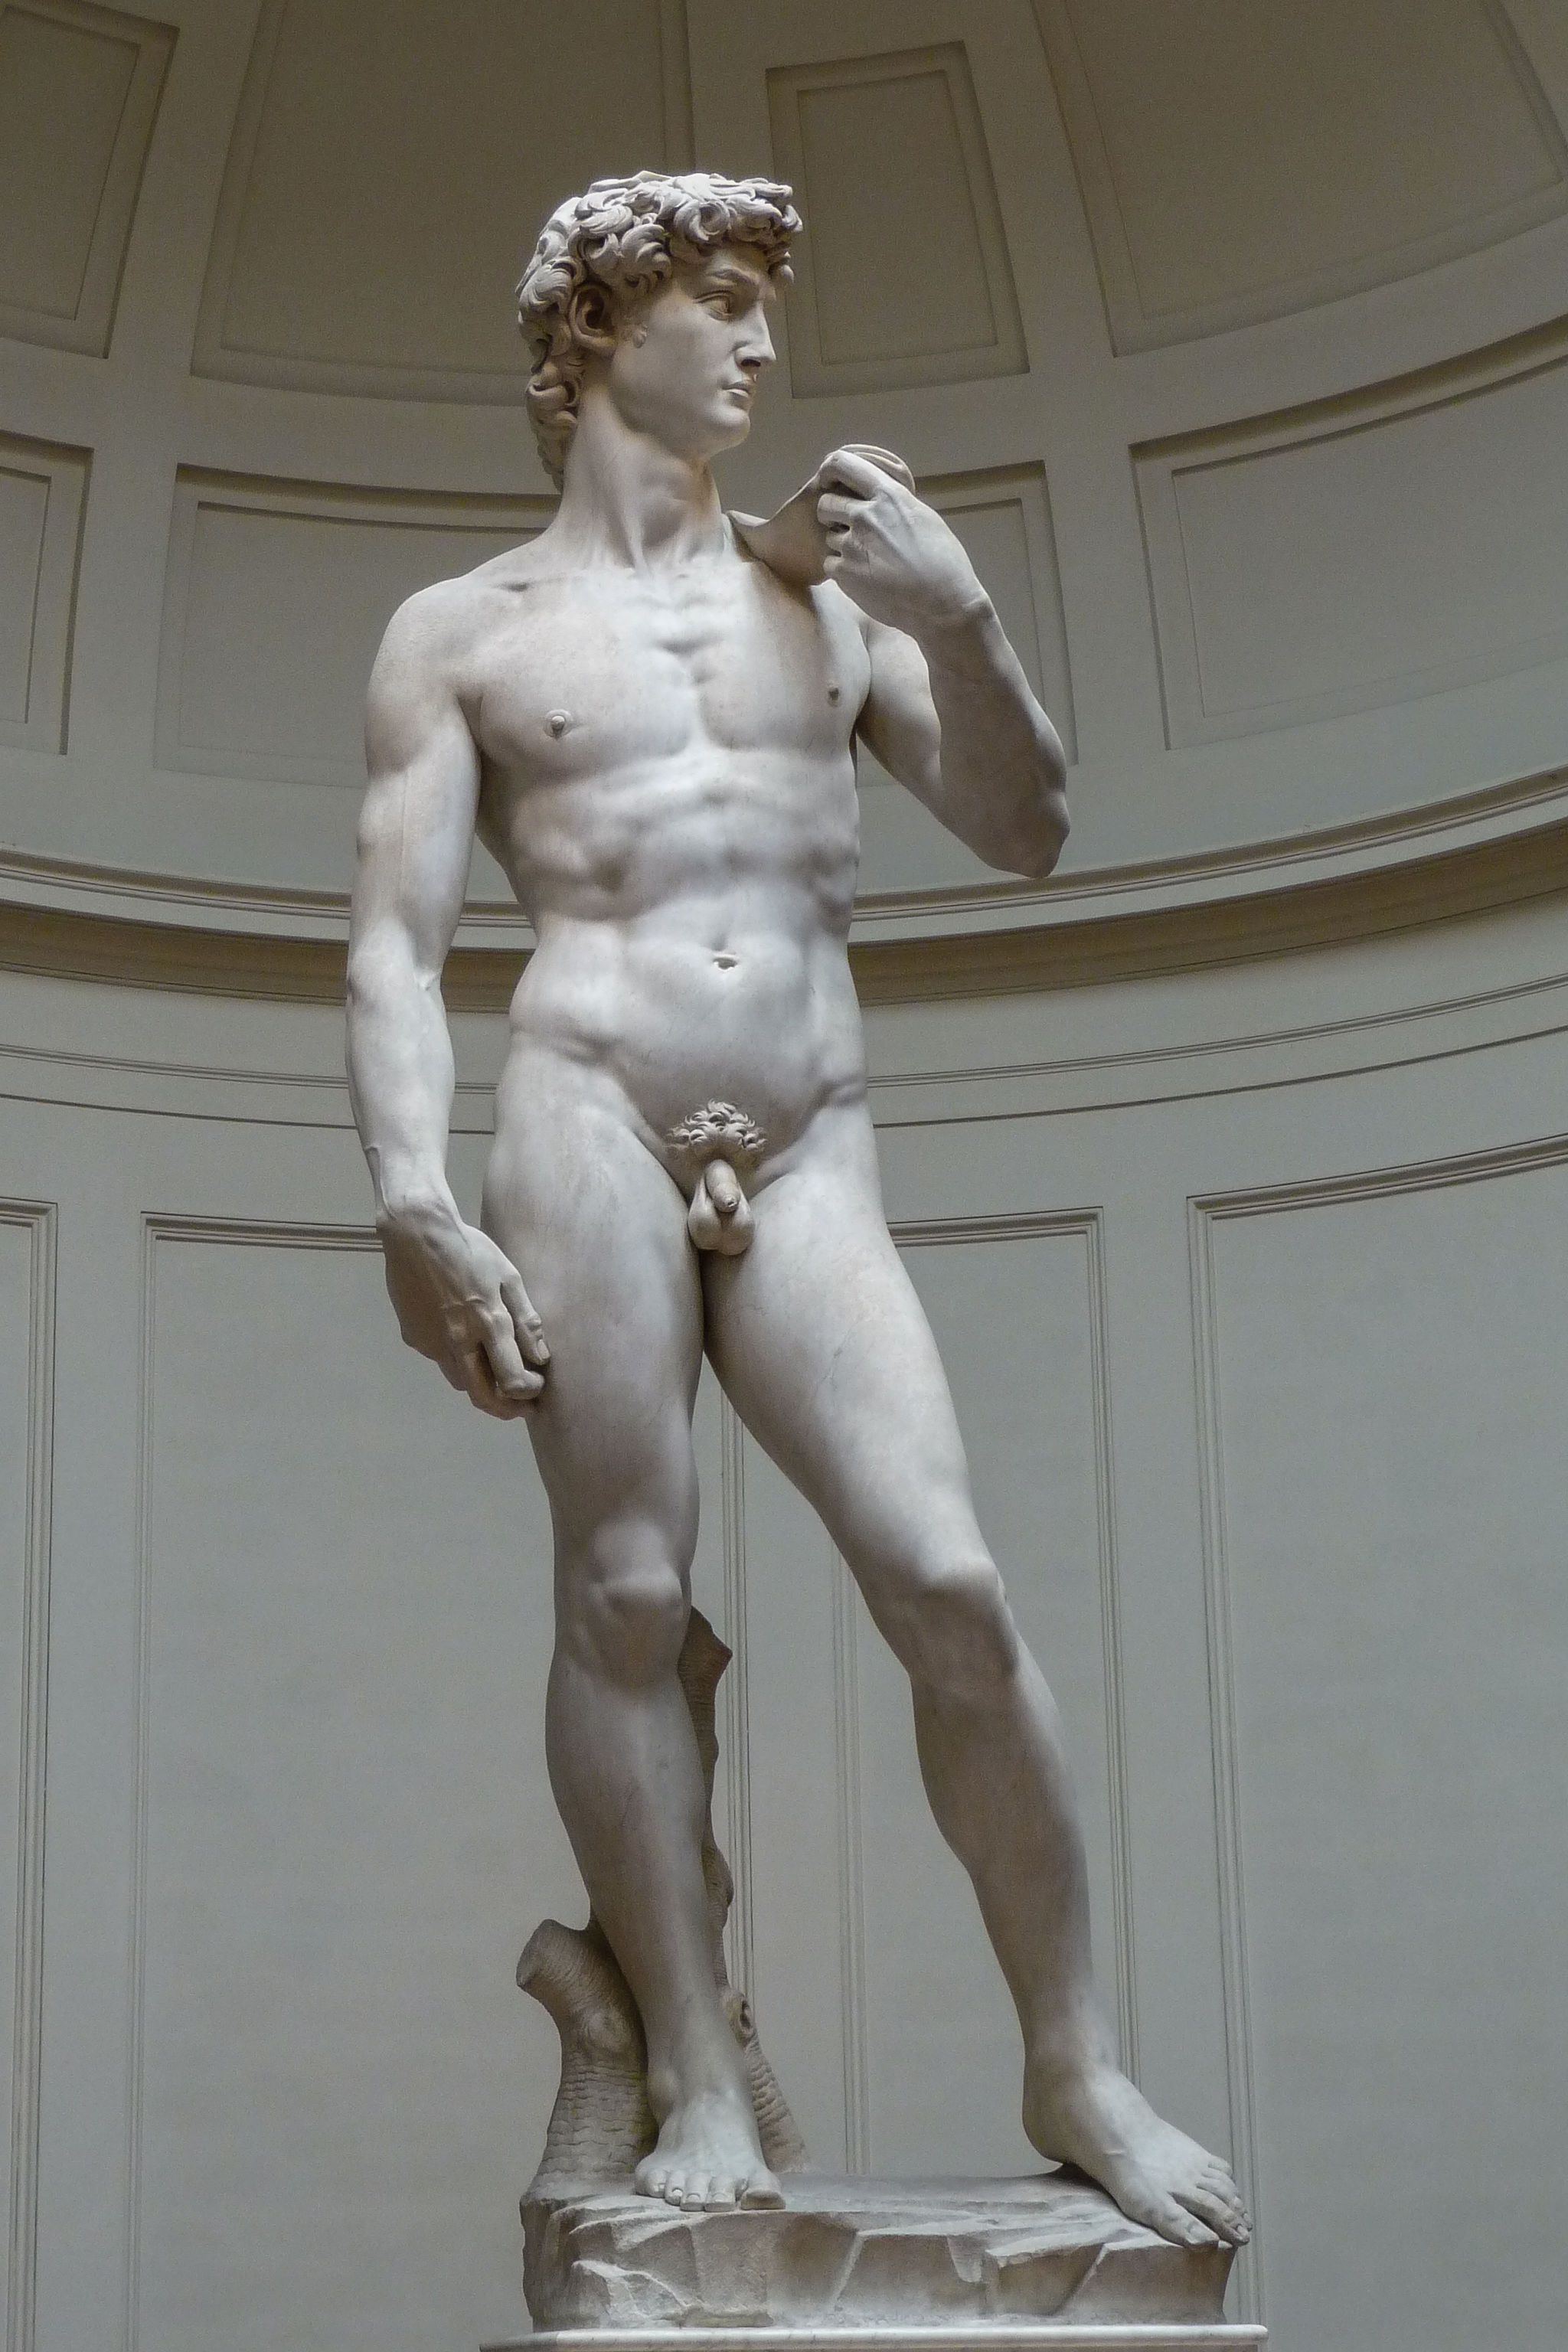
\includegraphics[width=0.30\textwidth]{figures/michelangelo_david} \\
\LARGE{Readymades} &  & \LARGE{Custommades}
\end{tabular}
\end{center}

\vf
\vspace{0.3in}
\TINY{\url{https://commons.wikimedia.org/wiki/File:Duchamp_Fountaine.jpg}}\\
\TINY{\url{https://commons.wikimedia.org/wiki/File:\%27David\%27_by_Michelangelo_JBU0001.JPG}}

\end{frame}
%%%%%%%%%%%%%%%%%%%%%%%%%%
\begin{frame}

Big data $\rightarrow$ repurposed data
\pause
\begin{itemize}
\item good things
\item bad things
\end{itemize}

\end{frame}
%%%%%%%%%%%%%%%%%%%%%%%%%%


\end{document}
